\thispagestyle{lichsutoanhocnone}
\pagestyle{lichsutoanhoc}
\graphicspath{{../lichsutoanhoc/pic/}}
\everymath{\color{lichsutoanhoc}}
\blfootnote{$^1$\color{lichsutoanhoc}Hà Nội.}
\begingroup
\AddToShipoutPicture*{\put(0,616){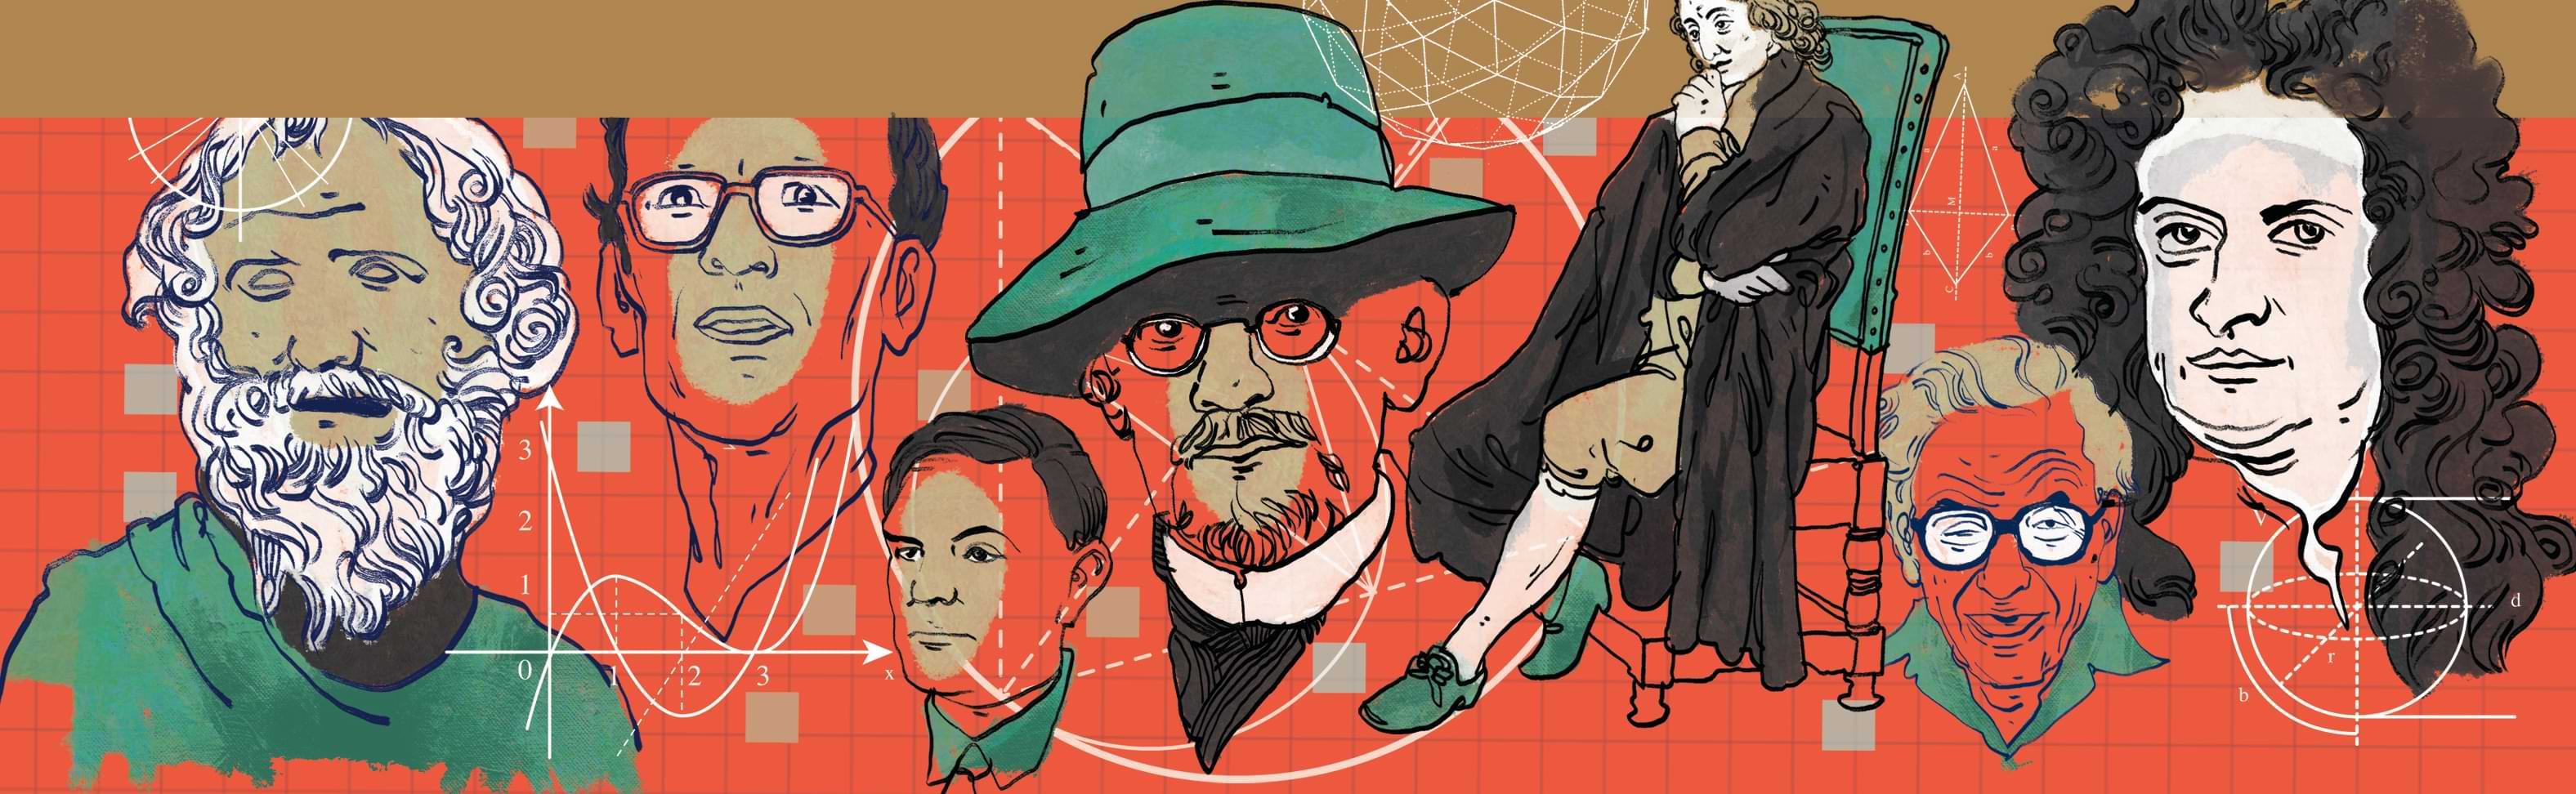
\includegraphics[width=19.3cm]{../bannerlichsu}}}
\AddToShipoutPicture*{\put(72,520){
\includegraphics[scale=1]{../tieude.pdf}}}
\centering
\endgroup

\vspace*{190pt}

\begin{multicols}{2}
	\begin{figure}[H]
		\vspace*{5pt}
		\centering
		\captionsetup{labelformat= empty, justification=centering}
		
\includegraphics[width= 1\linewidth]{1}
		\caption{\small\textit{\color{lichsutoanhoc}Hình $1$. Áp phích cho bộ phim Indiana Jones and the Dial of Destiny ($2023$).}}
		\vspace*{-10pt}
	\end{figure}
	Bộ phim mới nhất trong loạt phim khảo cổ Indiana Jones mang tên \textit{Indiana Jones and the Dial of Destiny} vừa ra mắt trong năm $2023$. Nội dung phim xoay quanh một thiết bị cổ đại được Archimedes thiết kế (bề mặt của nó là nền của áp phích quảng cáo phim) có thể dự đoán các đứt gãy thời gian cho phép con người du hành ngược về quá khứ. Thiết bị này được dựa trên nguyên bản là một thiết bị được các nhà khảo cổ phát hiện từ đầu thế kỷ $20$. Tuy không có khả năng giúp chúng ta di chuyển xuyên thời gian, câu chuyện thực tế về nó cũng vẫn có nhiều điều thú vị và độc đáo mà chúng ta sẽ cùng tìm hiểu trong bài viết này.
	\vskip 0.1cm
	$\pmb{1.}$ \textbf{\color{lichsutoanhoc}Quá trình phát hiện và những nghiên cứu ban đầu}
	\vskip 0.1cm
	Năm $1900$, các thợ lặn mò bọt biển ở gần đảo Antikythera, Hy Lạp phát hiện một con tàu đắm từ thời Hy Lạp cổ đại. Các nhà khảo cổ học đã tiến hành trục vớt và mang lên bờ nhiều hiện vật. Trông số đó, có một khối bằng đồng kích cỡ ngang với một quyển từ điển lớn nhưng không được ai để ý đến. Vài tháng sau, khối này vỡ ra cho thấy nhiều thiết bị dạng bánh răng chính xác chỉ to bằng cỡ đồng xu. Tổng cộng có tất cả $82$ mảnh vỡ và đến nay vẫn chưa có câu trả lời hoàn thiện về việc chúng khớp với nhau như thế nào. Được đặt tên là thiết bị Antikythera, theo tên của hòn đảo nơi nó được phát hiện, cấu tạo và chức năng của nó vẫn là một câu hỏi lớn cho khoa học ngày nay.
	\begin{figure}[H]
		\vspace*{5pt}
		\centering
		\captionsetup{labelformat= empty, justification=centering}
		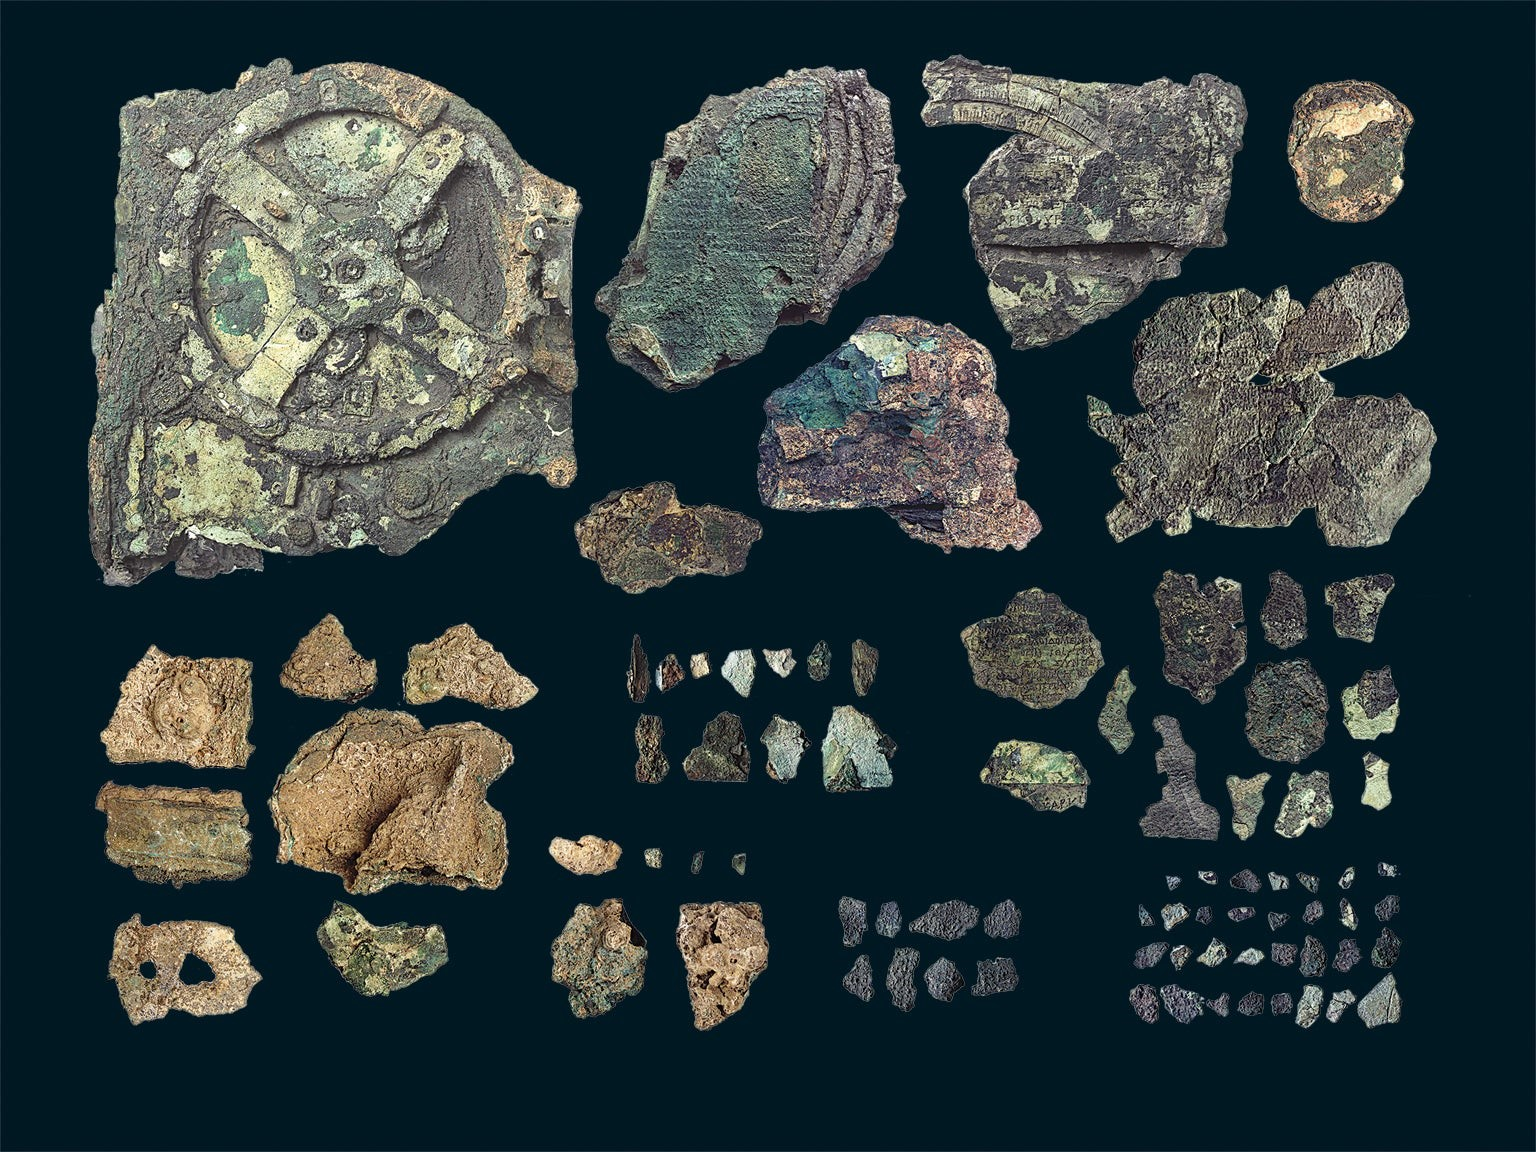
\includegraphics[width= 1\linewidth]{2}
		\caption{\small\textit{\color{lichsutoanhoc}Hình $2$. Các mảnh vỡ của thiết bị Antikythera được lưu trữ tại bảo tàng Athens.}}
		\vspace*{-10pt}
	\end{figure}
	Nỗ lực đầu tiên để khám phá bí ẩn của thiết bị Antikythera được nhà nghiên cứu ngôn ngữ cổ đại Albert Rehm tiến hành. Trong khoảng những năm $1905$ và $1906$, ông đã phát hiện các con số xuất hiện trên cùng một mảnh vỡ: $19$, $76$ và $223$. Đây là các con số đặc biệt có liên quan đến thiên văn học. Chu kỳ Meton (đặt tên theo một nhà thiên văn học Hy Lạp cổ đại) bao gồm $19$ năm, tức là $235$ chu kỳ giao hội của Mặt Trăng (chu kỳ giao hội là khoảng thời gian mà Mặt Trăng xuất hiện lại ở cùng vị trí so với Trái Đất, xấp xỉ bằng $27{,}32166$ ngày). Sau mỗi chu kỳ Meton, pha (tròn/khuyết) của Mặt Trăng lại xuất hiện lại ở cùng vị trí vào đúng một ngày cố định trong lịch Mặt trời. Do năm dương lịch gần với $365\dfrac{1}{4}$ ngày, một giá trị không nguyên nên nhà toán học Hy Lạp Callippus đã đưa ra chu kỳ $76$ năm (gấp $4$ chu kỳ của Meton). Trong khi đó, chu kỳ \textit{saros} (theo cách gọi của người Babylon cổ đại) kéo dài $223$ tháng là chu kỳ mà nguyệt thực lặp lại ở cùng thời điểm trong năm và cùng vị trí so với Trái Đất. Dựa trên các con số này, Rehm đã đề xuất rằng thiết bị Antikythera có chức năng tính toán thiên văn, nhưng mô hình ông đưa ra không đúng do thiếu các dữ liệu.
	\vskip 0.1cm
	Đến những năm $1950$, Derek de Solla Price, một nhà vật lý chuyển sang nghiên cứu lịch sử khoa học, bắt đầu tiến hành nghiên cứu sâu hơn về các mảnh vỡ và sử dụng các phương pháp mới như chụp ảnh X--quang. Từ các dữ liệu này, Price cho rằng thiết bị Antikythera có đến ít nhất $27$ bánh răng bên trong (con số ngày nay là lớn hơn $30$). Do sự ăn mòn vì nằm hàng nghìn năm dưới đáy biển, số lượng răng của mỗi bánh khó có thể xác định được một cách chính xác. Đồng thời, trong các hình ảnh X--quang $2$ chiều mà Price thu được, hình ảnh các bánh răng cũng chồng lấn lên nhau một cách phức tạp. Theo quan sát của ông, bánh răng lớn nhất có thể có $223$ hoặc $225$ răng. Price cũng phát hiện được một bánh răng với $127$ răng mà ông cho là có liên quan đến chu kỳ Meton $19$ năm ($19$ năm có $235$ chu kỳ tròn khuyết của Mặt Trăng nhưng nếu tính chu kỳ Mặt Trăng theo sự lặp lại vị trí trên bầu trời của nó thì $19$ năm có $254=2\times127$ chu kỳ dạng này, sự khác biệt là do quỹ đạo dạng ellipse của Mặt Trăng quanh Trái Đất). Bánh răng này hoạt động trong một tổ hợp các bánh răng liên kết với nhau và được điều khiển bằng một bánh răng có $38$ răng thông qua các bánh răng trung gian (cần nhớ rằng $38=19\times2$). Theo mô hình của Price, thiết bị Antikythera có thể đã được sử dụng để xác định vị trí của Mặt trời, Mặt Trăng và các hành tinh cho một ngày cụ thể trong quá khứ cũng như tương lai.
	\begin{figure}[H]
		\vspace*{-5pt}
		\centering
		\captionsetup{labelformat= empty, justification=centering}
		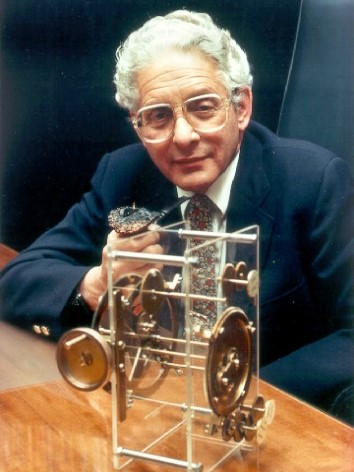
\includegraphics[width= 0.72\linewidth]{3}
		\caption{\small\textit{\color{lichsutoanhoc}Derek de Solla Price ($1922-1983$)}}
		\vspace*{-5pt}
	\end{figure}
	Người sử dụng chỉ cần quay một tay quay để vận hành thiết bị và các bánh răng sẽ vận hành các kim trên một bề mặt tương tự với mặt la bàn. Price đã đạt một bước tiến lớn khi xác định được vị trí tương đối giữa các khối lớn cũng như cấu tạo tổng quát với các mặt la bàn ở trước và sau. Quá trình nghiên cứu miệt mài suốt $16$ năm của Price được ông tổng kết trong cuốn sách năm $1974$ mang tên \textit{Các bánh răng từ người Hy Lạp}. Theo Price, thiết bị Antikythera có thể coi là một trong những hiện vật quan trọng nhất để hiểu về khoa học kỹ thuật Hy Lạp cổ đại, mang lại nhiều thông tin hơn những di vật bằng đá hay gốm trong các bảo tàng. Nhiều khía cạnh đời sống của nền văn minh này vẫn chưa sáng tỏ, đặc biệt là các công cụ cơ khí và kim loại được sử dụng trong các lĩnh vực đời sống khác nhau, từ nông nghiệp đến xây dựng. Price mất năm $1983$, khi mà các câu hỏi về lịch sử khoa học ông đặt ra vẫn chưa có lời giải đáp. 
	\begin{figure}[H]
		\vspace*{-5pt}
		\centering
		\captionsetup{labelformat= empty, justification=centering}
		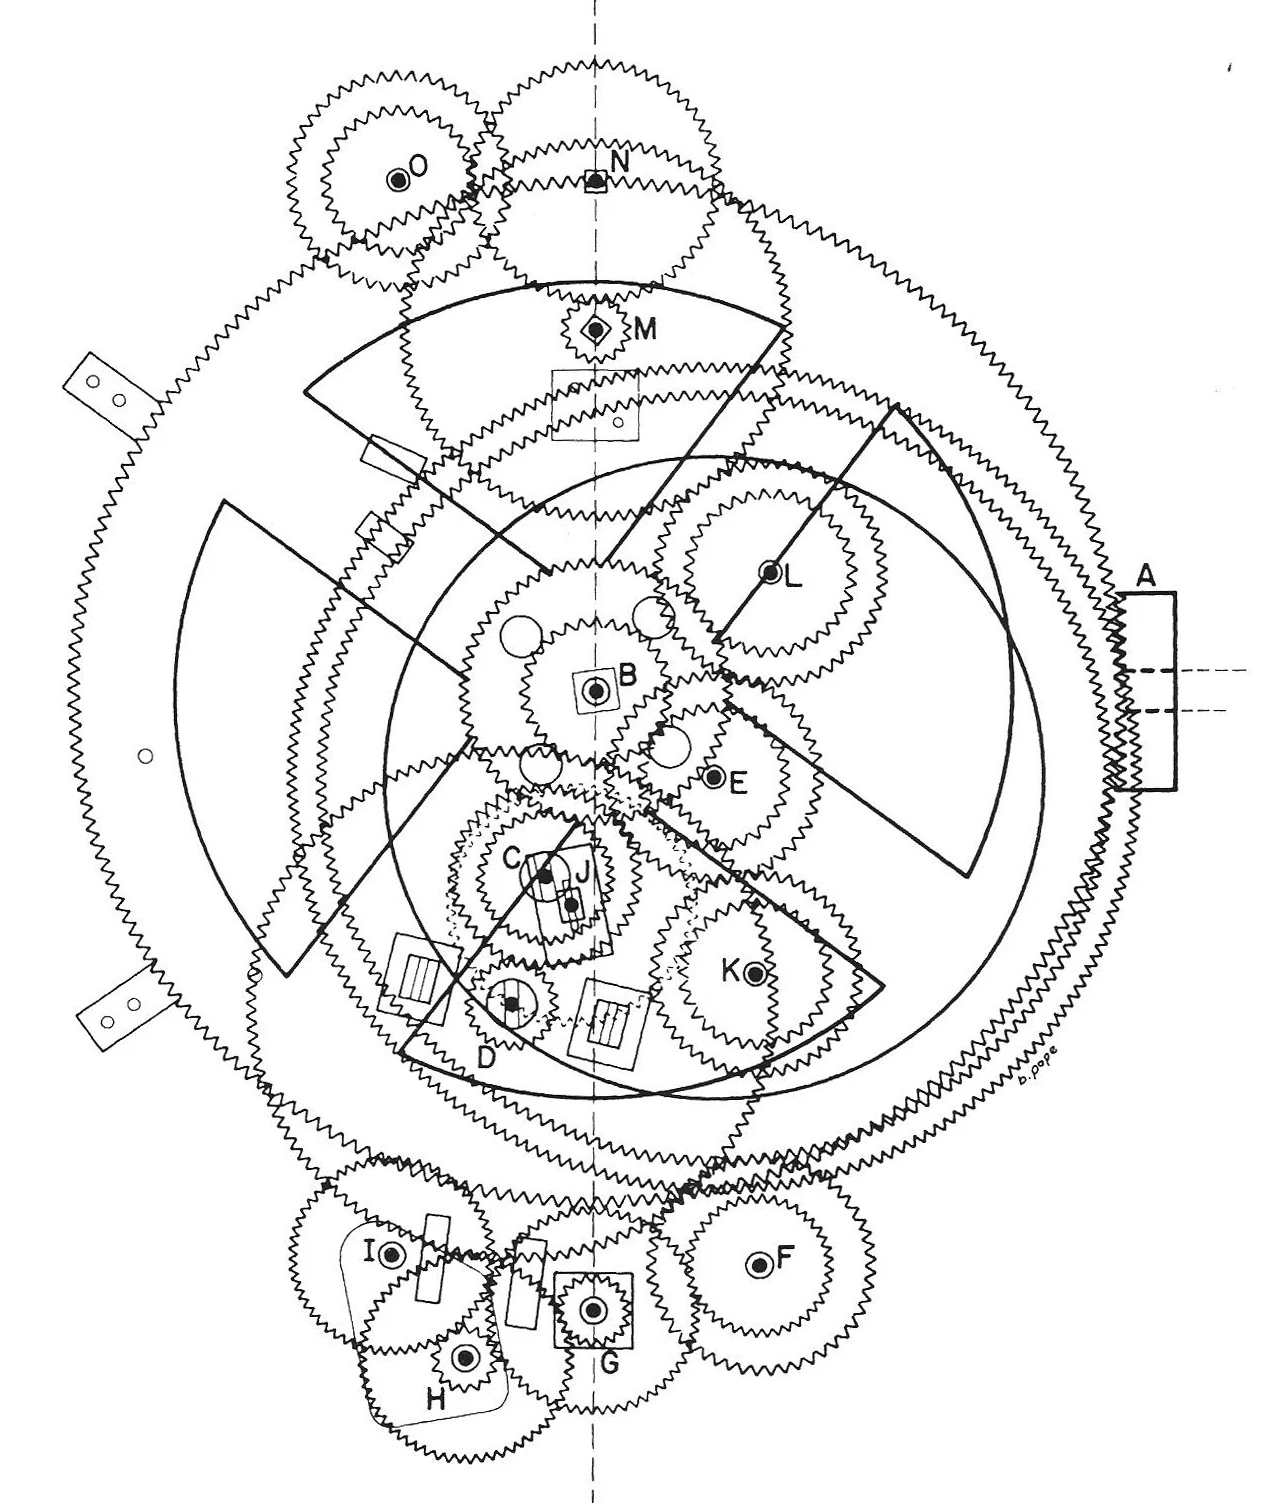
\includegraphics[width= 0.85\linewidth]{4}
		\caption{\small\textit{\color{lichsutoanhoc}Hình $3$. Đề xuất của Price về cấu tạo các bánh răng của thiết bị Antikythera}}
		\vspace*{-10pt}
	\end{figure}
	Sau Price, Michael Wright, một nhà nghiên cứu ở Bảo tàng Khoa học London lại tiến hành chụp X--quang các mảnh vỡ lần nữa với sự cộng tác của nhà lịch sử máy tính Allan Bromley nhằm mục đích cho ra một mô hình chính xác hơn. Wright đã chỉ ra nhiều điểm không đúng với thực tế trong mô hình của Price. Ông cũng đã tiến hành phục dựng lại thiết bị Antikythera với các bánh răng bằng đồng thau có độ dày chỉ từ $1$ đến $2$ mm giống như các hiện vật đã được phát hiện. Wright đã phát hiện được số răng chính xác cho một số bánh răng mới cũng như làm rõ hơn một số chức năng của thiết bị. Thiết bị phục dựng của ông cũng cho thấy tính khả thi của việc chế tạo một thiết bị thiên văn như vậy ở thời cổ đại.
	\begin{figure}[H]
		\vspace*{-5pt}
		\centering
		\captionsetup{labelformat= empty, justification=centering}
		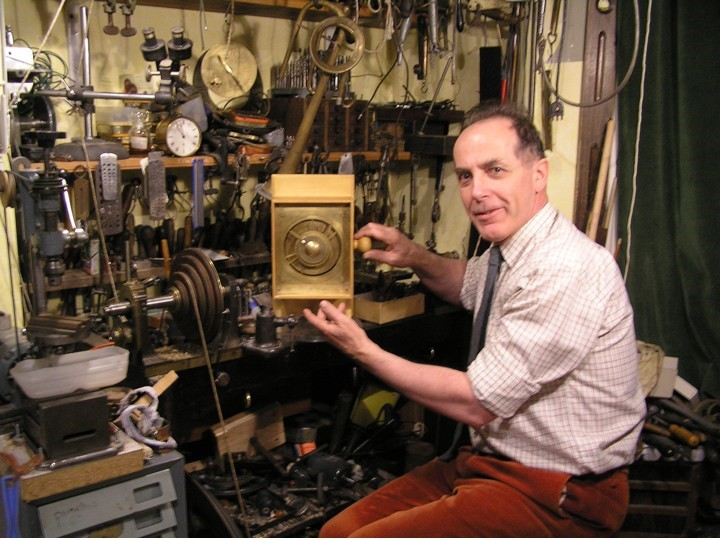
\includegraphics[width= 1\linewidth]{5}
		\caption{\small\textit{\color{lichsutoanhoc}Hình $4$. Wright và mô hình thiết bị Antikythera do ông chế tạo.}}
		\vspace*{-10pt}
	\end{figure}
	$\pmb{2.}$ \textbf{\color{lichsutoanhoc}Giả thuyết mới về cấu tạo chi tiết và vận hành}
	\vskip 0.05cm
	Năm $2005$, thiết bị Antikythera lại được chụp X--quang lần thứ ba, sử dụng công nghệ chụp cắt lớp CT với một máy chụp đặc biệt còn đang được thí nghiệm. Các kết quả chụp được cải thiện nhờ một thuật toán xử lý hình ảnh mới của Hewlett--Packard (HP) để tăng cường các chi tiết trên bề mặt trong ảnh. Những dữ liệu mới này cho phép nhà toán học người Anh Tony Freeth và nhà nghiên cứu lịch sử khoa học Alexander Jones (Viện  Nghiên cứu Thế giới Cổ đại, Đại học New York) tiến hành các nghiên cứu sâu hơn về các chi tiết vận hành của thiết bị Antikythera.
	\vskip 0.1cm
	Hình chụp mới cho thấy bánh răng chính trong thiết bị có $223$ răng, ứng với chu kỳ saros. Việc này khẳng định rằng thiết bị cổ đại của chúng ta không chỉ dự đoán chuyển động của các thiên thể mà còn có thể dự đoán nhật thực và nguyệt thực. Bánh răng chính sẽ quay một kim đồng hồ trên một đĩa xoắn ốc với $4$ vòng xoáy được chia làm tổng cộng $223$ phần theo $223$ tháng của chu kỳ {saros}. Đồng thời, Freeth và Jones cũng phát hiện ra chức năng của $4$ bánh răng khác nằm trong phạm vi của bánh răng chính: chúng cho phép tính các chuyển động biến thiên của Mặt Trăng. Trong thực tế, Mặt Trăng có quỹ đạo hình ellipse quanh Trái Đất chứ không phải quỹ đạo tròn. Người Hy Lạp cổ đại không biết đến dạng quỹ đạo này nên đã mô phỏng nó bằng một dạng quỹ đạo kết hợp hai chuyển động tròn gọi là epicycle.
	\begin{figure}[H]
		\vspace*{-5pt}
		\centering
		\captionsetup{labelformat= empty, justification=centering}
		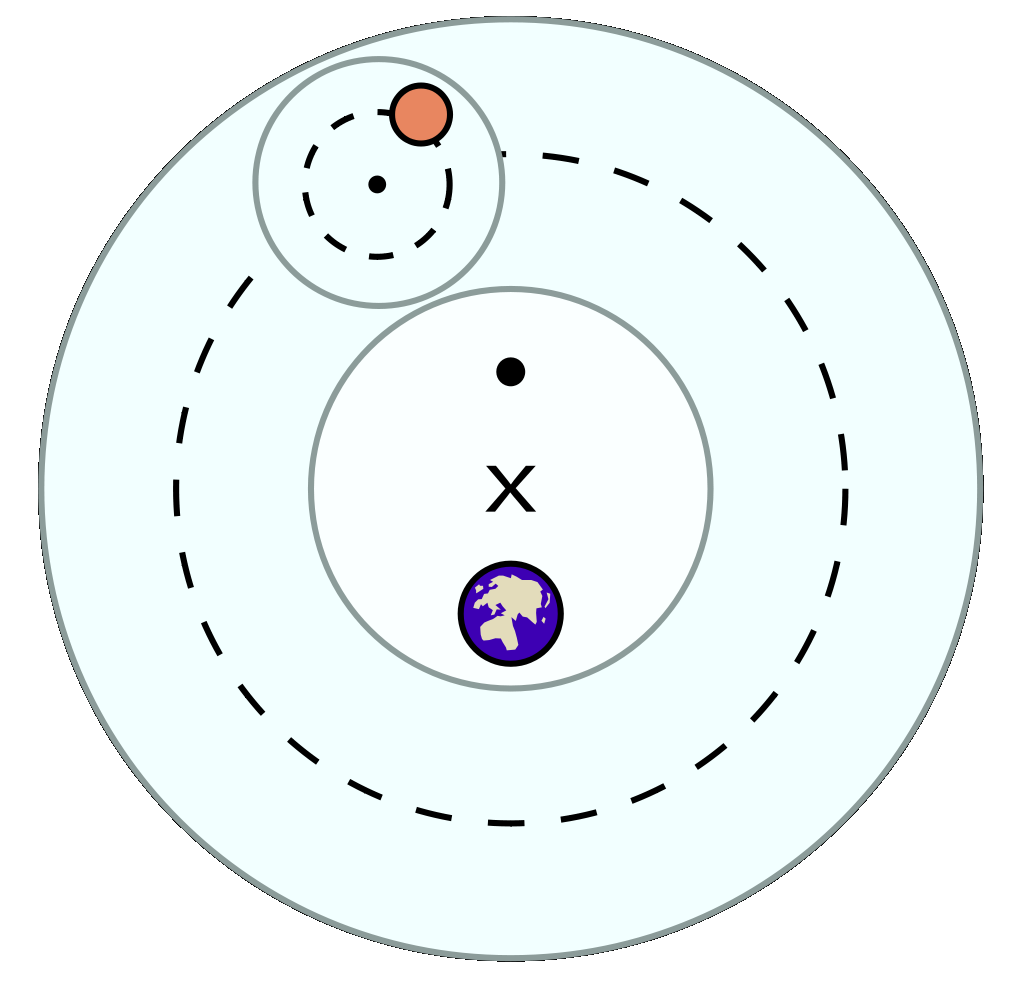
\includegraphics[width= 0.8\linewidth]{6}
		\caption{\small\textit{\color{lichsutoanhoc}Hình $5$. Dạng quỹ đạo epicycle theo mô tả của nhà toán học Hy Lạp cổ đại Ptolemy. Một hành tinh sẽ chuyển động tròn trên một đường tròn mà tâm của nó cũng chuyển động tròn trên một quỹ đạo có tâm ở điểm đánh dấu X gần với Trái Đất. Nếu nhìn từ điểm (.) thì hành tinh có vận tốc góc không đổi. Mô hình phức tạp này được sinh ra nhằm khớp chuyển động tròn với các số liệu thiên văn quan sát được thời đó. Nó chỉ rời khỏi lịch sử khi các định luật Kepler được phát hiện rất nhiều thế kỷ sau đó.}}
		\vspace*{-10pt}
	\end{figure}
	Dạng quỹ đạo này được điều khiển trong thiết bị Antikythera nhờ một cơ chế mà Wright đã phát hiện ra. Các bánh răng nhỏ hơn có một kim trên bề mặt gắn vào một lỗ trên bánh răng chính. Tuy nhiên, do trục của chúng hơi lệch nhau chỉ khoảng $1$ mm, hệ thống sẽ cho ra các chuyển động biến thiên so với chuyển động tròn. Các hình ảnh chụp X--quang CT thể hiện rõ cơ chế này. Các bánh răng xung quanh sẽ không có trục cố định mà trục của chúng được gắn vào vành của bánh răng $223$ răng. Công bố của Freeth và nhóm của ông năm $2006$ đã cho thấy kết cấu này cùng với lý thuyết về chuyển động dạng epicycle được sử dụng để hiển thị chuyển động của Mặt Trăng trên mặt sau của thiết bị Antikythera.
	\vskip 0.1cm
	Quá trình giải thích mặt trước của thiết bị khó khăn hơn nhiều. Mảnh vỡ lớn nhất là bánh răng chính có chu kỳ quay ứng với một năm khi hoạt động. Nó không phải là một đĩa phẳng như các bánh răng chính mà có $4$ nan hoa cùng nhiều kết nối với các phần khác thông qua các trục.
	\vskip 0.1cm
	Trước đó, dựa trên ý tưởng của Price, Wright đã đề xuất rằng hệ thống bánh răng ở mặt trước được sử dụng để tính các chu kỳ của các hành tinh xung quanh Mặt trời, bao gồm $5$ hành tinh đã biết từ thời Hy Lạp cổ đại: sao Thủy, sao Kim, sao Hỏa, sao Mộc và sao Thổ, theo dạng chu kỳ epicycle. Ông đã tự chế tạo một mô hình bằng đồng thau từ thiết kế của mình. Tuy nhiên, mô hình của Wright rất phức tạp với tám đầu ra đồng trục trong khi phần mặt trước của thiết bị Antikythera không có mức độ phức tạp như vậy. Dữ liệu chụp CT năm $2005$ còn cho biết thêm nhiều đoạn văn bản trên các mảnh vỡ mà trước đó chưa được phát hiện. Năm $2016$, Alexander Jones, một giáo sư lịch sử thiên văn ở Đại học New York đã tìm ra mô tả về việc chuyển động của Mặt trời và các hành tinh được biểu diễn bằng các vành với viên bi chuyển động từ những văn tự này. Câu hỏi đặt ra là nếu phần mặt trước của thiết bị không hoạt động theo những gì mà Wright đã nghĩ thì cơ chế tính toán chu kỳ thực sự của nó là như thế nào?
	\vskip 0.1cm
	Trong những phần văn bản còn sót lại từ thiết bị, người ta phát hiện ra các con số $462$ cho sao Kim và $442$ cho sao Thổ. Những con số này không khớp với các chu kỳ được biết đến cho các hành tinh này trong thiên văn học cổ đại. Trong một nghiên cứu mới gần đây, Freeth và nhóm nghiên cứu của mình đã đề xuất rằng các con số này xuất phát từ hai chu kỳ: $289$ chu kỳ giao hội trong $462$ năm cho sao Kim và $427$ chu kỳ giao hội trong $442$ năm cho sao Thổ. Theo đó, những chu kỳ này được tính toán từ các chu kỳ đã biết cho những hành tinh trên sử dụng công thức của Parmenides, một nhà toán học Hy Lạp cổ đại sống vào thế kỷ thứ $6$ đến thứ $5$ trước Công nguyên. Giả sử có một đại lượng $\theta$ mà ta đã biết các giá trị gần đúng của nó là $\dfrac{p}{q}$ và $\dfrac{r}{s}$. Khi đó, một số giá trị xấp xỉ khác của nó có thể được thiết lập dưới dạng $\dfrac{p+kr}{q + ks}$ hoặc $\dfrac{kp + r}{kq + s}$.
	\begin{figure}[H]
		\vspace*{-5pt}
		\centering
		\captionsetup{labelformat= empty, justification=centering}
		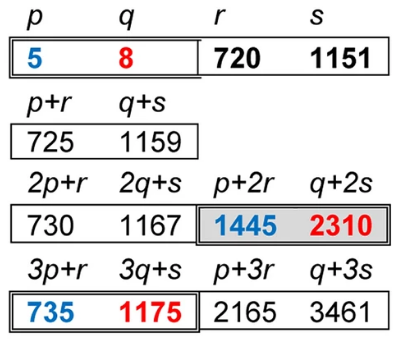
\includegraphics[width= 1\linewidth]{7}
		\caption{\small\textit{\color{lichsutoanhoc}Hình $6$. Các chu kỳ được sinh từ hai chu kỳ $(5,8)$ và $(720,1151)$ cho sao Kim. Các chu kỳ có thể phân tích thành các thừa số nguyên tố nhỏ hơn $100$ được tô màu.}}
		\vspace*{-10pt}
	\end{figure}
	Việc lựa chọn chu kỳ nào để sử dụng trong các chu kỳ được sinh ra phụ thuộc vào các yếu tố như tính chính xác, khả năng phân tích ra thừa số nguyên tố và tính tối ưu khi thiết kế cơ khí. Chu kỳ được chọn cần phải đủ chính xác để khớp với các giá trị đã biết cho các hành tinh như sao Kim hay sao Thổ. Đồng thời, nó cũng phải cho phép việc phân tích ra thừa số nguyên tố dễ dàng để đảm bảo rằng số răng của các bánh răng trong hệ thống không quá lớn gây khó khăn trong chế tạo. Ví dụ, với sao Kim, chu kỳ $(5,8)$ tuy đơn giản nhưng lại có độ chính xác không cao. Trong khi đó, chu kỳ $(720,1151)$ chính xác hơn đã được biết đến từ thời Babylon cổ đại lại chứa số $1151$ không phân tích được thành tích các thừa số nguyên tố nhỏ. Mặt khác, để tối ưu thiết kế, các hành tinh khác nhau cần phải chia sẻ một số bánh răng nếu chúng có cùng các thừa số nguyên tố, làm giảm số lượng bánh răng giúp việc chế tạo dễ dàng hơn. Trong khi chu kỳ $(289,462)=(17^2,2\times3\times7\times11)$ được sử dụng cho sao Kim thì chu kỳ $(427,442)=(7\times61,2\times13\times17)$ được chọn cho sao Thổ. Sự xuất hiện của các thừa số nguyên tố chung ví dụ như $17$ giúp cho một số bánh răng có thể được sử dụng chung giữa các hành tinh, làm giảm mức độ phức tạp của việc thiết kế và chế tạo.
	\begin{figure}[H]
		\vspace*{-5pt}
		\centering
		\captionsetup{labelformat= empty, justification=centering}
		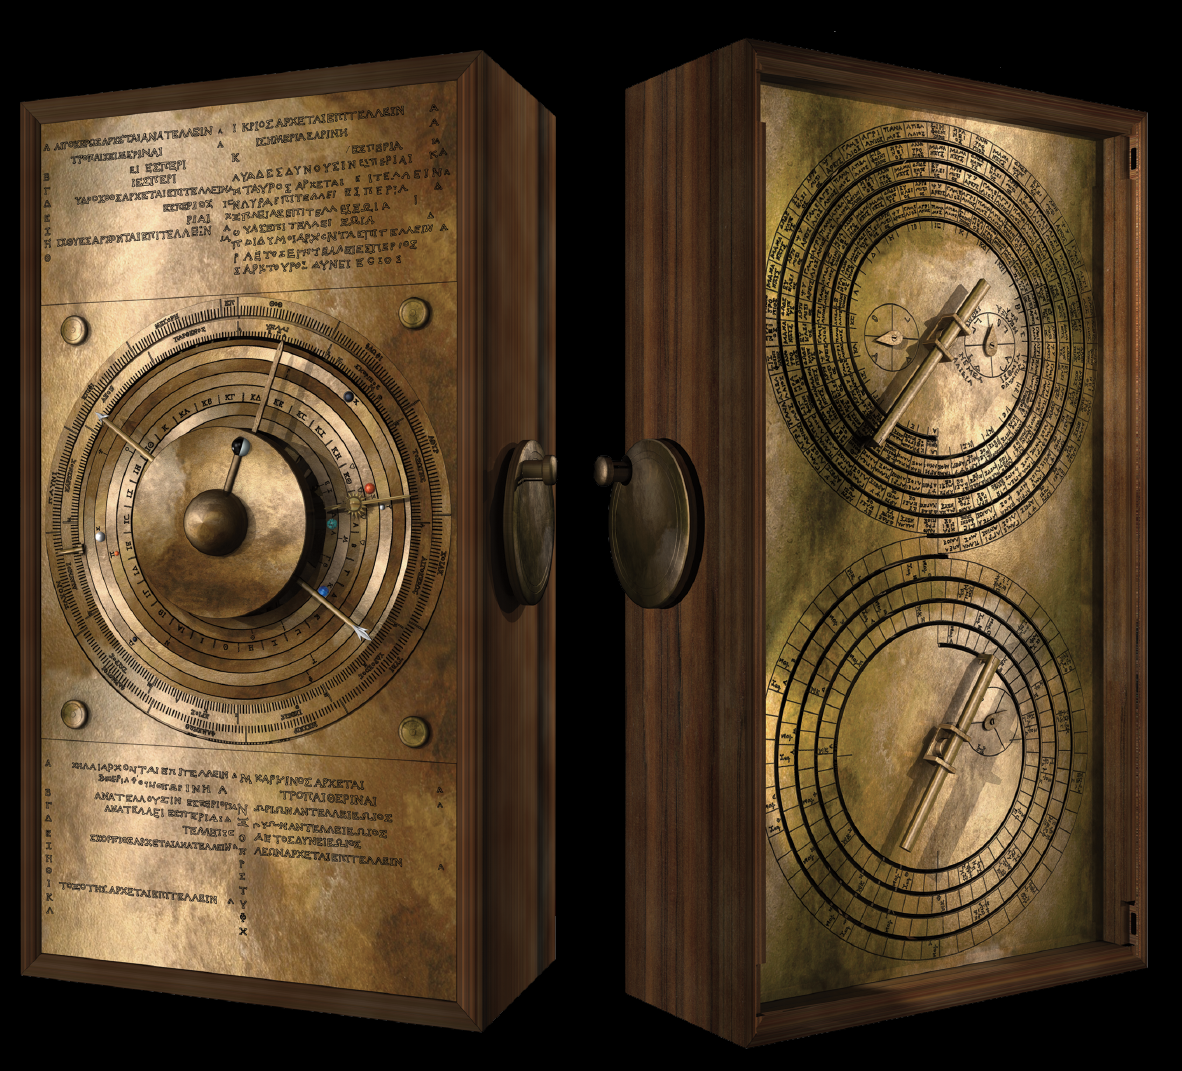
\includegraphics[width= 1\linewidth]{8}
		\caption{\small\textit{\color{lichsutoanhoc}Hình $7$. Hình ảnh phục dựng phía ngoài thiết bị Antikythera. Mặt trước (bên trái trong hình) biểu diễn chuyển động của Mặt trời và các hành tinh. Mặt sau (bên phải trong hình) biểu diễn chuyển động của Mặt Trăng cùng chu kỳ nguyệt thực.}}
		\vspace*{-10pt}
	\end{figure}
	Dựa trên các giả thuyết này cũng như các đặc điểm của một số mảnh vỡ, nhóm nghiên cứu 
	\end{multicols}
	\begin{figure}[H]
		\vspace*{5pt}
		\centering
		\captionsetup{labelformat= empty, justification=centering}
		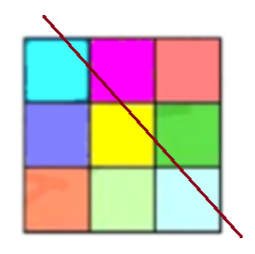
\includegraphics[width= 1\linewidth]{9}
		\caption{\small\textit{\color{lichsutoanhoc}Hình $8$. Mô hình cấu tạo bên trong của thiết bị Antikythera theo Tony Freeth. $1)$ Kim chỉ cho Mặt Trăng. $2)$ Kim chỉ cho các tiết điểm của Mặt Trăng (điểm quỹ đạo Mặt Trăng cắt Hoàng đạo). $3)$ Cơ chế cho chuyển động của Mặt trời. $4)$ Bản hình chữ nhật. $5)$ Bánh răng đầu vào, gắn với tay quay. $6)$ Bánh răng $53$ răng cho chuyển động của Mặt Trăng. $7)$ Cột đỡ. $8)$ Bánh răng $38$ răng. $9)$ Bánh răng chính. $10)$ Trục đầu ra cho chuyển động biến thiên của Mặt Trăng. $11)$ Bảng chữ nhật chính. $12)$ Bánh răng $127$ răng cho chuyển động trung bình của Mặt Trăng. $13)$ Cơ chế trục và lỗ để điều khiển chuyển động biến thiên của Mặt Trăng. $14)$ Bánh răng $188$ răng (hàn vào bánh răng $233$ răng).}}
		\vspace*{-10pt}
	\end{figure}
	\begin{multicols}{2}
	của Jones cũng đã đề xuất các chu kỳ được sử dụng cho các hành tinh còn lại cùng một thiết kế của phần mặt trước theo các chu kỳ này. Tuy chưa thể hoàn toàn khẳng định do nhiều mảnh vỡ vẫn đang thất lạc, mô hình mới này có thể được coi là gần nhất với thiết kế thật của thiết bị trong số các giả thuyết hiện có. 
	\vskip 0.1cm
	$\pmb{3.}$ \textbf{\color{lichsutoanhoc}Bí ẩn về nguồn gốc}
	\vskip 0.1cm
	Thiết bị cổ đại trong bộ phim Indiana Jones được chính Archimedes chế tạo, còn với thiết bị Antikythera trong thực tế, chúng ta vẫn chưa thể có kết luận chắc chắn với nhiều giả thuyết khác nhau. Trong các ghi chép của học giả Cicero thời La Mã, Archimedes đã chế tạo một thiết bị hình cầu mô phỏng chuyển động của Mặt trời, Mặt Trăng và các hành tinh. Bản thân Wright từ các mô tả còn sót lại đã phục dựng một thiết bị như vậy. Có rất nhiều khả năng, thiết bị Antikythera được ra đời sau đó là kết quả của một quá trình phát triển từ thiết bị của Archimedes.
	\begin{figure}[H]
		\vspace*{-5pt}
		\centering
		\captionsetup{labelformat= empty, justification=centering}
		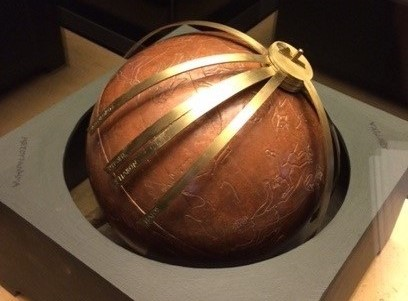
\includegraphics[width= 1\linewidth]{10}
		\caption{\small\textit{\color{lichsutoanhoc}Hình $9$. Quả cầu của Archimedes do Wright dựng lại.}}
		\vspace*{-5pt}
	\end{figure}
	\vskip 0.1cm
	\begin{wrapfigure}{l}{0.45\linewidth}
%		\vspace*{-5pt}
		\centering
		\captionsetup{labelformat= empty, justification=centering}
		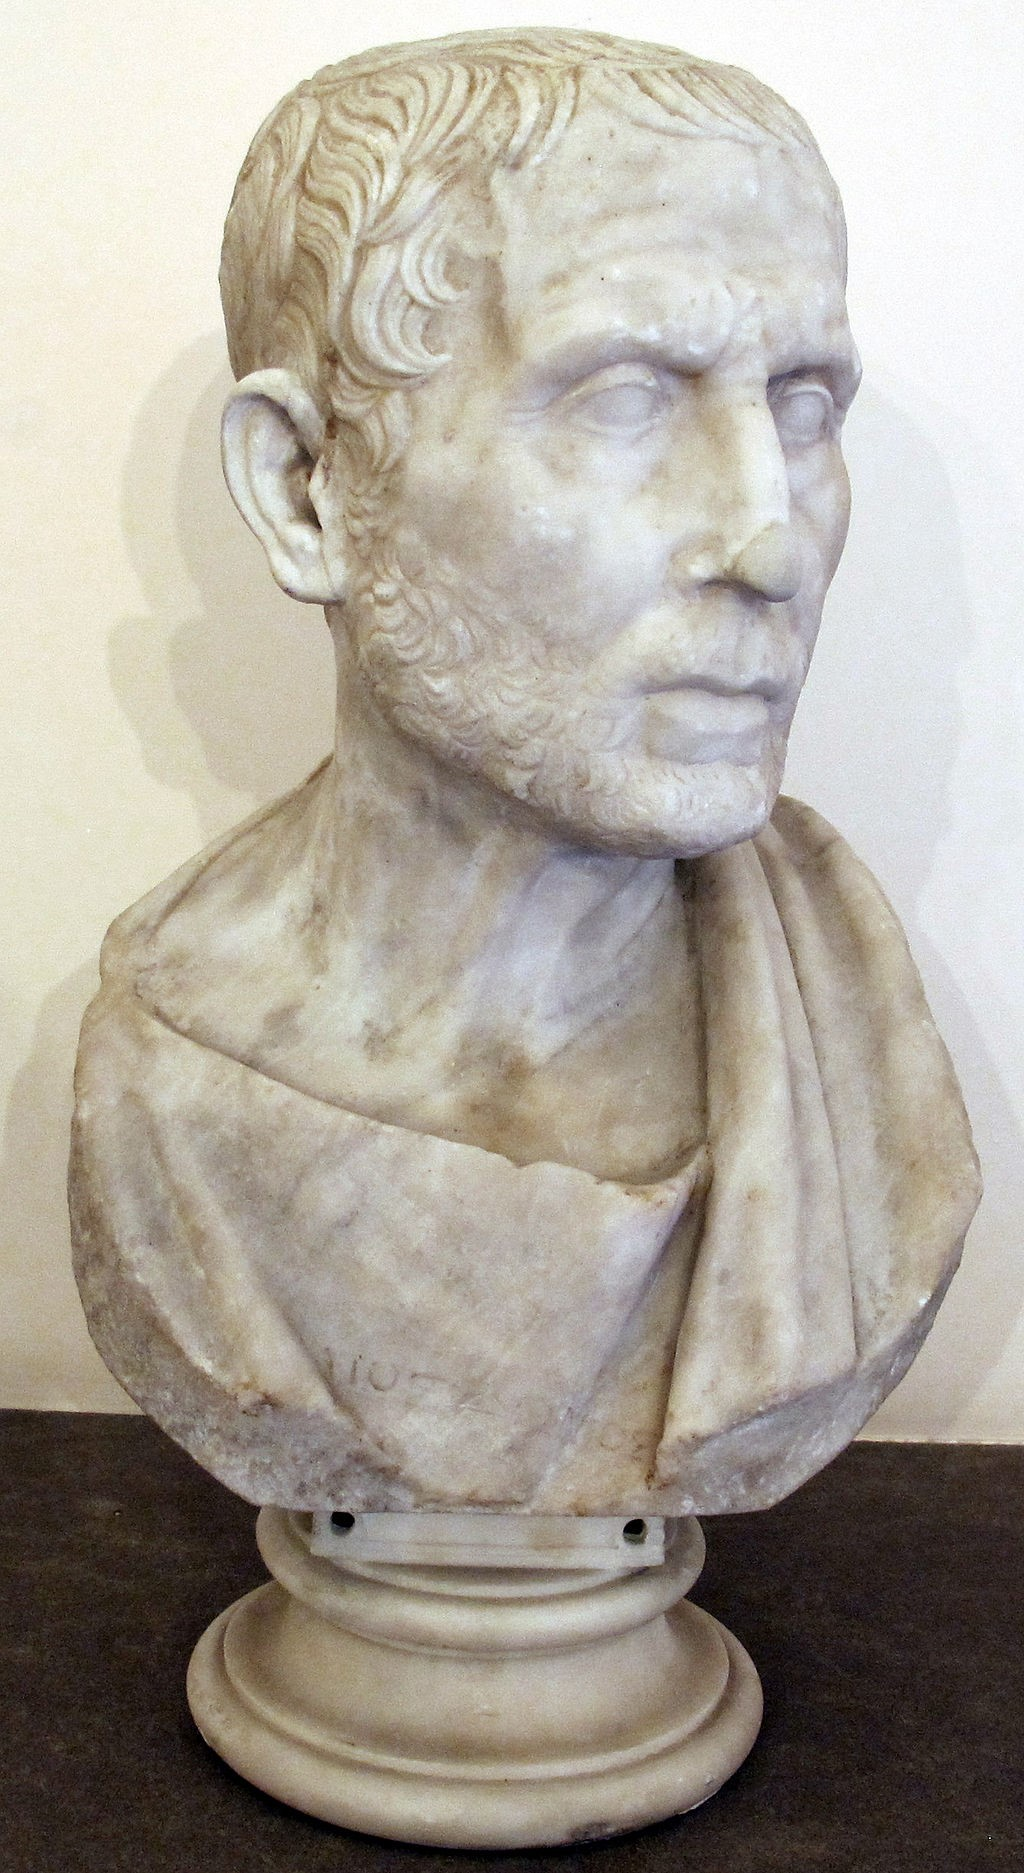
\includegraphics[width= 1\linewidth]{11}
		\caption{\small\textit{\color{lichsutoanhoc}Hình $10$. Tượng Posidonius ở Bảo tàng khảo cổ học Naples (Italy).}}
		\vspace*{-10pt}
	\end{wrapfigure}
	Mặt khác, Cicero cũng nhắc đến một thiết bị có chức năng tương tự thiết bị Antikythera khi ông ở đảo Rhodes. Nó được nhà toán học Hy Lạp Posidonius chế tạo. Do con tàu chở thiết bị Antikythera bị đắm khi đang trên tuyến đường từ Rhodes về đất liền, việc thiết bị này liên quan đến Posidonius là rất có khả năng. Đồng thời, đảo Rhodes còn là nơi mà nhà toán học và thiên văn học Hipparchus, cha đẻ của lượng giác, từng sinh sống vài thập kỷ trước Posidonius nên mối liên hệ đến Hipparchus cũng là một khả năng có thể xảy ra. Nếu không có thêm những dữ kiện khảo cổ mới (hiện vật hoặc văn bản), nguồn gốc chính xác của thiết bị Antikythera vẫn là một vấn đề còn bỏ ngỏ.
	\vskip 0.1cm
	$\pmb{4.}$ \textbf{\color{lichsutoanhoc}Lời kết}
	\begin{figure}[H]
		\vspace*{-10pt}
		\centering
		\captionsetup{labelformat= empty, justification=centering}
		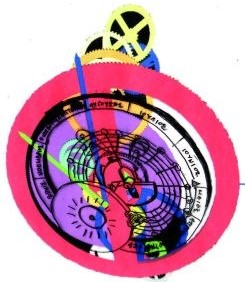
\includegraphics[width= 0.75\linewidth]{12}
		\caption{\small\textit{\color{lichsutoanhoc}Thiết bị Antikythera. Tranh của Dionysios Kriaris, một nhà toán học ở Athens, Hy Lạp.}}
		\vspace*{-10pt}
	\end{figure}
	Thiết bị Antikythera và những nghiên cứu xung quanh nó cho thấy một khía cạnh hoàn toàn mới về toán học và khoa học thời Hy Lạp cổ đại với các thiết bị cơ khí chính xác ở mức độ đáng kinh ngạc. Trước đó, thiết bị cơ khí chính xác sử dụng bánh răng sớm nhất được biết đến là một đồng hồ Mặt trời và lịch có nguồn gốc Byzantine từ thế kỷ thứ $6$ Công nguyên, với cấu tạo đơn giản hơn nhiều so với thiết bị Antikythera. Những nội dung trong bài viết này chỉ mang tính giới thiệu sơ lược, các độc giả muốn tìm hiểu nhiều hơn các chi tiết liên quan đến thiết bị Antikythera có thể xem thêm ở các tài liệu trong phần tài liệu tham khảo. Các nghiên cứu khảo cổ học trong tương lai sẽ còn tiếp tục mang đến những phát hiện mới xung quanh thế giới cổ đại, đặc biệt về toán học và khoa học của nhân loại trong giai đoạn này.
	\vskip 0.1cm
	\textbf{\color{lichsutoanhoc}Tài liệu tham khảo}
	\vskip 0.1cm
	[$1$] Freeth, T. An Ancient Greek Astronomical Calculation Machine Reveals New Secrets. \textit{Scientific American}, $326(1)$, $24-33$ ($2022$).
	\vskip 0.1cm
	[$2$] Freeth, T., Bitsakis, Y., Moussas, X., Seiradakis, J. H., Tselikas, A., Mangou, H., \ldots\, Edmunds, M. G. Decoding the ancient Greek astronomical calculator known as the Antikythera Mechanism. \textit{Nature}, $444(7119)$, $587-591$ ($2006$). \url{https://doi.org/10.1038/nature05357}
	\vskip 0.1cm
	[$3$] Freeth, T., Higgon, D., Dacanalis, A., MacDonald, L., Georgakopoulou, M., \& Wojcik, A. A Model of the Cosmos in the ancient Greek Antikythera Mechanism. \textit{Scientific Reports}, $11(1)$, ($2021$). \url{https://doi.org/10.1038/s41598-021-84310-w}
	\vskip 0.1cm
	[$4$] Jones, A. \textit{A portable cosmos : revealing the Antikythera Mechanism, scientific wonder of the ancient world}. New York, Ny: Oxford University Press  ($2017$).
	\vskip 0.1cm
	[$5$] Lin, J.--L., \& Yan, H.--S. \textit{Decoding the Mechanisms of Antikythera Astronomical Device}. Springer ($2015$).
\end{multicols}